\documentclass[10pt]{amsart}
\usepackage{amsmath}
\usepackage{amsthm}
\usepackage{tikz}
\usepackage{multicol}
\usetikzlibrary{automata, positioning, arrows}

\theoremstyle{definition}
\newtheorem{definition}{Definition}[section]
\newtheorem{theorem}{Theorem}[section]

\title{The Word Problem for Automata Groups}
\author{Arden Rasmussen}
\date{\today}

\newcommand{\Z}{\mathbb{Z}}
\renewcommand{\sp}{\textvisiblespace}

\begin{document}

\maketitle

\section{Finite State Automata}%
\label{sec:finite_state_automata}

We will first begin with some definitions that are used in the description of
automatic groups. Firstly $\Sigma$ is the finite set of \textit{letters}, this
is commonly called the \textit{alphabet}. Commonly $\sp\in\Sigma^*$ is defined
as always mapping to the identity. Then the free monoid generated by
$\Sigma$ will be denoted $\Sigma^*$, and the elements of $\Sigma^*$ are
commonly called \textit{words} or \textit{strings}, and it possesses an
identity as the \textit{empty word} which will be denoted as $\epsilon$. The
free monoid $\Sigma^*$ can be though of as the set of all possible combinations
of letters in $\Sigma$. For example consider the alphabet
\begin{align*}
  \Sigma=\left\{a,b\right\}\Rightarrow\Sigma^*=\left\{a,b,aa,ab,ba,bb,\ldots\right\}.
\end{align*}

The product of two strings $u,v\in\Sigma^*$ is denoted simply as $uv$ and
represents the concatenation of the strings. We will also make use of the
notation $|w|$ to mean the length of a string for some string $w\in\Sigma^*$. A
subset of $\Sigma^*$ is called a \textit{language}, and a subset of
$\Sigma^*\times\Sigma^*$ is called a \textit{relation}.

In our case we can commonly view the alphabet $\Sigma$ to be the set of
generators $X$ for some group $G$ along with their inverses, so we can write
$\Sigma=X\cup X^{-1}$. Then $\Sigma^*$ is the set of products of
generators, of arbitrary length.

A Finite State Automaton is defined as the quintuple $\left(\Sigma, S, s_0,
  \delta, F\right)$. Where $\Sigma$ is the alphabet of symbols, $S$ is a
non-empty finite set of states, $s_0$ is the initial state such that $s_0\in
S$, $\delta$ is the state-transition function $\delta:S\times\Sigma\rightarrow
S$, and $F$ is the finite set of states $F\subseteq S$, and $F$ could be the
empty set.

Since the automaton that we will be working with are deterministic, then there
is exactly one output for every input. So we can consider the automaton $A$ as
a mapping $A:\Sigma^*\rightarrow S$.

\begin{figure}[htpb]
  \begin{center}
    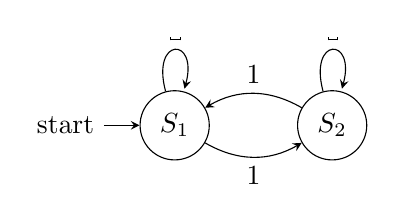
\begin{tikzpicture}[scale=1, transform shape,->,>=stealth]
      \node[state, initial] at (-1,0) (s1) {$S_1$};
      \node[state] at (1,0) (s2) {$S_2$};
      \draw (s1) edge[bend right, below] node{$1$} (s2);
      \draw (s2) edge[bend right, above] node{$1$} (s1);
      \draw (s1) edge[loop above, above] node{$\sp$} (s1);
      \draw (s2) edge[loop above, above] node{$\sp$} (s2);
    \end{tikzpicture}
  \end{center}
  \caption{Very simple Finite state automata}%
  \label{fig:auto_ex}
\end{figure}

Consider the Finite State Automaton presented in figure \ref{fig:auto_ex}. For
this automaton $\Sigma=\left\{0, 1\right\}$, $S=\left\{S_1,S_2\right\}$,
$s_0=S_1$, and
\begin{align*}
  \delta(s, l) = \begin{cases}
    s & \text{if }l=\sp \\
    S_1 & \text{if }s=S_2\text{ and }l=1\\
    S_2 & \text{if }s=S_1\text{ and }l=1
  \end{cases}.
\end{align*}

Note that the explicit format for $\delta$ can be relatively complex, so it is
common to express the transition function as a table. Thus the transition table
for this automaton is given in Table \ref{tab:auto_ex}.

\begin{table}[htpb]
  \centering
  \caption{Transition table for Figure\ref{fig:auto_ex}.}
  \label{tab:auto_ex}
  \begin{tabular}{c||c|c}
    $\delta$ & \sp & 1\\
    \hline\hline
    $S_1$ & $S_1$ & $S_2$\\
    \hline
    $S_2$ & $S_2$ & $S_1$\\
  \end{tabular}
\end{table}

We can use this table to determine the output of the finite state automaton.
Let us consider the example where $w\in\Sigma^*$, with $w=111\sp\sp1$. Running the
automaton with this input of $w$ we see that each stage is described below
\begin{multicols}{2}
  \begin{enumerate}
    \item $s=S_1$, $w=111\sp\sp1$.
    \item $s=S_2$, $w=11\sp\sp1$.
    \item $s=S_1$, $w=1\sp\sp1$.
    \item $s=S_2$, $w=\sp\sp1$.
    \item $s=S_2$, $w=\sp1$.
    \item $s=S_2$, $w=1$.
    \item $s=S_1$, $w=\epsilon$.
  \end{enumerate}
\end{multicols}

Thus after the automaton has been run on the input of $w$ the output of the
automaton is $S_1$. We can see that this automaton is actually representative
of $\Z/2\Z$, when we replace $S_1$ with $0$, ad $S_2$ with $1$.

To construct an automaton from a group, let us consider the group $D_4$, the
generators for $D_4$ are given as $\langle a,b | a^4=1, b^2=1,
(ab)^2=1\rangle$. We will denote the states, as the most reduced form of their
generators, thus $S=\left\{e,a,a^2,a^3,b,ab,a^2b,a^3b\right\}$. Now we consider
our $X=\left\{a,b\right\}$. Then we find
$\Sigma=\left\{a,a^{-1},b,b^{-1}\right\}$. And finally the transition table for
$D_4$ is given in table \ref{tab:d4};

\begin{table}[htpb]
  \centering
  \caption{Transition table for $D_4$}
  \label{tab:d4}
  \begin{tabular}{c||c|c|c|c}
    $\delta_{D_4}$ & $a$ & $a^{-1}$ & $b$ & $b^{-1}$\\
    \hline\hline
    $e$ & $a$ & $a^3$ & $b$ & $b$\\
    $a$ & $a^2$ & $e$ & $a^3b$ & $a^3b$\\
    $a^2$ & $a^3$ & $a$ & $a^2b$ & $a^2b$\\
    $a^3$ & $e$ & $a^2$ & $ab$ & $ab$\\
    $b$ & $ab$ & $a^3b$ & $e$ & $e$\\
    $ab$ & $a^2b$ & $b$ & $a^3$ & $a^3$\\
    $a^2b$ & $a^3b$ & $ab$ & $a^2b$ & $a^2b$\\
    $a^3b$ & $b$ & $a^2b$ & $a$ & $a$\\
  \end{tabular}
\end{table}

Using this table, and the states, we can construct the diagram representing the
automaton for $D_4$.

\begin{figure}[htpb]
  \begin{center}
    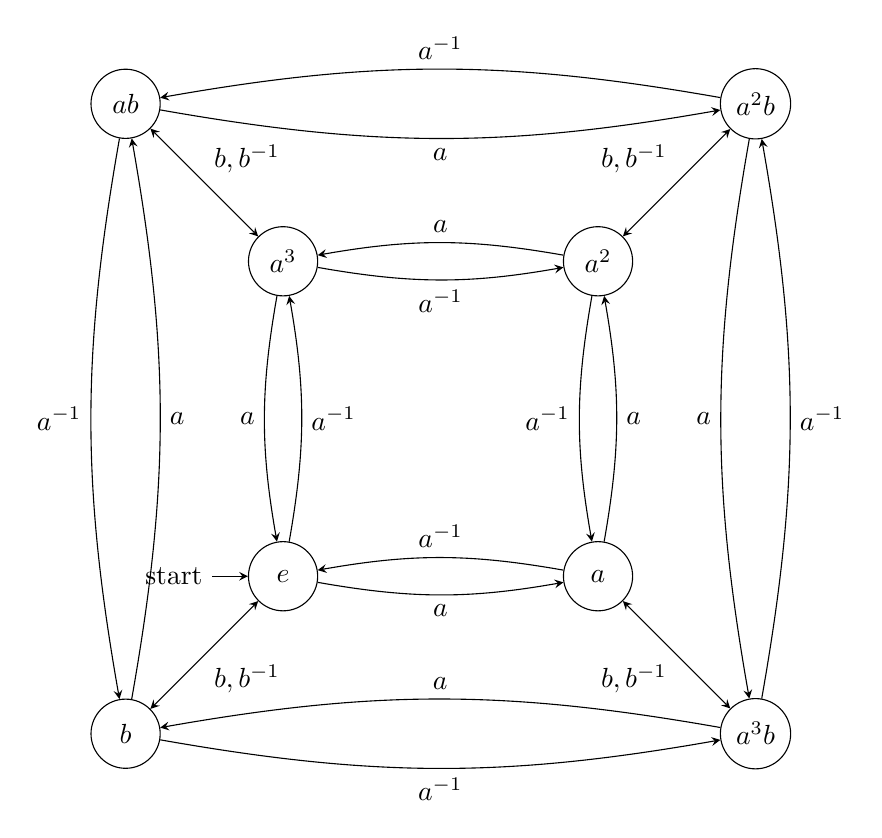
\begin{tikzpicture}[scale=1, transform shape,->,>=stealth]
      \node[state, initial] at (-2,-2) (e) {$e$};
      \node[state] at (2,-2) (a) {$a$};
      \node[state] at (2,2) (a2) {$a^2$};
      \node[state] at (-2,2) (a3) {$a^3$};

      \node[state] at (-4,-4) (b) {$b$};
      \node[state] at (-4,4) (ab) {$ab$};
      \node[state] at (4,4) (a2b) {$a^2b$};
      \node[state] at (4,-4) (a3b) {$a^3b$};

      \draw (e) edge[bend right=10, below] node{$a$} (a);
      \draw (a) edge[bend right=10, right] node{$a$} (a2);
      \draw (a2) edge[bend right=10, above] node{$a$} (a3);
      \draw (a3) edge[bend right=10, left] node{$a$} (e);
      \draw (e) edge[bend right=10, right] node{$a^{-1}$} (a3);
      \draw (a3) edge[bend right=10, below] node{$a^{-1}$} (a2);
      \draw (a2) edge[bend right=10, left] node{$a^{-1}$} (a);
      \draw (a) edge[bend right=10, above] node{$a^{-1}$} (e);

      \draw (e) edge[below right,<->] node{$b,b^{-1}$} (b);
      \draw (a) edge[below left,<->] node{$b,b^{-1}$} (a3b);
      \draw (a2) edge[above left,<->] node{$b,b^{-1}$} (a2b);
      \draw (a3) edge[above right,<->] node{$b,b^{-1}$} (ab);

      \draw (b) edge[bend right=10, right] node{$a$} (ab);
      \draw (ab) edge[bend right=10, below] node{$a$} (a2b);
      \draw (a2b) edge[bend right=10, left] node{$a$} (a3b);
      \draw (a3b) edge[bend right=10, above] node{$a$} (b);
      \draw (ab) edge[bend right=10, left] node{$a^{-1}$} (b);
      \draw (a2b) edge[bend right=10, above] node{$a^{-1}$} (ab);
      \draw (a3b) edge[bend right=10, right] node{$a^{-1}$} (a2b);
      \draw (b) edge[bend right=10, below] node{$a^{-1}$} (a3b);
    \end{tikzpicture}
  \end{center}
  \caption{Finite state automaton for $D_4$}%
  \label{fig:d4}
\end{figure}

With this automaton representation of $D_4$ we can consider any sequence of
generators $w\in\Sigma^*$, and determine the reduced representation of this
element, we just need to apply the automaton as we did in the prior example.
Lets consider $w=aabaaba^{-1}bb^{-1}aab$. By applying the same process as
before, we find that $w=a^3b$.

\section{The Word Problem}\label{sec:the_word_problem}

The common form of the word problem is given two representations of elements in
a set, determine if the two expressions represent the same element. As we saw
in the previous section, the finite state automaton can represent a mapping
from elements of $\Sigma^*$ to states $S$, where we defined each state as
equivalent to an element of the group. Thus the formulation of the word problem
in the context of Automatic groups is

\begin{theorem}\label{thm:twp}
  For a finitely generated group $G$, and two representations of an element in
  that group $w,u,\in\Sigma^*$. And an automaton $A=\left(\Sigma,G,e\right)$.
  Then it is possible to state whether $w=u$.
\end{theorem}

An equivalent definition for the word problem is to consider it is a problem of
rewriting elements in some group $G$. For some set of generators $x, y,
z,\ldots$ for $G$, we introduce one letter for $x$ and another for $x^{-1}$. We
will then call these letters the alphabet $\Sigma$ for the problem. With this
definition every element in $G$ is represented in some way by a product
$abc\cdots pqr$ of symbols from $\Sigma$ of some length. The string of length
$0$ is the representative of the identity of $G$. With this construction the
question is to be able to recognize all different ways to express the identity
$e$ of $G$, given some relations.

At first this may appear trivial, to state weather two elements are the same,
or not. However, it has been proven that the word problem is not universally
solvable. That is to say, given some arbitrary group, it may not be possible to
say if two representations are the same element or not. However, given an
Automatic group it is solvable.

To get some intuition to the motivation of the word problem, consider for
$D_4$, $w=aababa^{-1}bbabbaab^{-1}a^{-1}b$ and
$u=aba^{-1}a^{-1}baaab^{-1}a^{-1}a^{-1}b$, although these appear very
different, these are actually equivalent and both $w$ and $u$ represent $e$.

\section{Cyclic Group of Order 3}%
\label{sec:cyclic_group_of_order_3}

Proving the word problem is solvable for the Cyclic group of order 3 is
relatively simple, and so we will use it to explain the concept more generally.

\begin{align}
  Z_3=\langle x \vert x^3 \rangle
\end{align}
In this group, our alphabet consists of $\Sigma=\left\{x,x^{-1}\right\}$, and
so $\Sigma^*$ is the set of all strings combining any number of the letters $x$
and $x^{-1}$. The first step is to write out the relations that we know. The
relations in $Z_3$ provide us with a list of strings that can be inserted or
canceled out whenever they appear in the string, without altering the
represented element of the group. In this case, the relations are listed below.
\begin{multicols}{2}
  \begin{enumerate}
    \item $xxx= e$\label{enum:z3:1}
    \item $xx^{-1}= e$\label{enum:z3:2}
    \item $x^{-1}x= e$\label{enum:z3:3}
    \item $x^{-1}x^{-1}x^{-1}= e$\label{enum:z3:4}
    \item $x^{-1}= xx$\label{enum:z3:5}
    \item $x^{-1}x^{-1}= x$\label{enum:z3:6}
  \end{enumerate}
\end{multicols}
The first relation is derived directly from the definition of $Z_3$. The second
and third come from the definition of an inverse of the element $x$. Relation
\ref{enum:z3:4} is a result that since the cube of $x$ is the identity, then so
is the cube of the inverse of $x$. Relation \ref{enum:z3:5} and \ref{enum:z3:6}
come as a result of multiplying by $e$, and from relation \ref{enum:z3:1},
expanding this out to be of the form $xxxx^{-1}$ and $xxxx^{-1}x^{-1}$
respectively, then by relation \ref{enum:z3:2} we cancel elements are are left
with $xx$ and $x$ respectively.

With these relations we can reduce any string to either by the empty string
$\epsilon$, $x$, or $xx$. And thus the word problem is solvable for $Z_3$. Let
us test this by considering $w=xxx^{-1}xx^{-1}x^{-1}xxxx$.
\begin{align*}
  w&=xxx^{-1}xx^{-1}x^{-1}xxxx\\
  (\ref{enum:z3:2})&\rightarrow xxxx^{-1}x^{-1}xxxx\\
  (\ref{enum:z3:1})&\rightarrow x^{-1}x^{-1}xxxx\\
  (\ref{enum:z3:3})&\rightarrow x^{-1}xxx\\
  (\ref{enum:z3:3})&\rightarrow xx\\
\end{align*}
Thus we see that $w=xx=x^2$.

\section{Automatic Group Structure}%
\label{sec:automatic_group_structure}

In group theory the Automatic groups are groups with additional structure
applied to them in the form of finite state automata. This additional structure
is required for the Knuth-Bendix method to be guaranteed to succeed, which will
be discussed further in section \ref{sec:kunth_bendix_method}.

Right now I need to read into more information about the structure associated
with automatic groups. And why it is necessary for the Knuth-Bendix method to
work. From the Internet:

\begin{quote}
  Let $G$ be a group and $A$ a finite set of generators. Then an
  \textit{automatic structure} of $G$ with respect to $A$ is a set of finite
  state automata:
  \begin{itemize}
    \item the \textit{word-acceptor}, which accepts for every element of $G$ at
      least one word in $A^*$ representing it.
    \item \textit{multipliers}, one for each $a\in A\cup\left\{1\right\}$,
      which accept a pair $\left(w_1,w_2\right)$ for words in $w_i$ accepted by the
      word-acceptor, precisely when $w_1a=w_2$ in $G$
  \end{itemize}
\end{quote}

From a paper:

\begin{quote}
  The group $G$ is said to be automatic with respect to the generating set $A$
  if there exist finite state automata $W$, $M_\$$ and $M_a$ for each $a\in A$,
  with the following properties.
  \begin{enumerate}
    \item $W$ has input alphabet $A$ and, for each $g\in G$, there is at least
      one element $w\in A^*$ with $w\in L(W)$ (the language accepted by $W$)
      and $\bar{w}=g$.
    \item For $a=\$$ and $a\in A$, $M_a$ has input alphabet $A^\dagger\times
      A^\dagger$, $M_a$ accepts only padded words over $A\times A$ and, for all
      $v,w\in A^*$, ${(v, w)}^\dagger\in L\left(M_a\right)$ if and only if
      $v,w\in L(W)$ and $\bar{v}\bar{a}=\bar{w}$.
  \end{enumerate}
\end{quote}

\section{Shortlex Ordering}%
\label{sec:shortlex_ordering}

Before we are able to use the Knuth-Bendix method, we need to have some notion
of ordering for our representations. In our case we will simply use shortlex
ordering. Shortlex ordering is alphabetical ordering, where shorter words are
considered smaller. So given the alphabet $\Sigma=\left\{x,y\right\}$. Then the
shortlex ordering is represented by
\begin{align*}
  \varepsilon<x<y<xx<xy<yx<yy<\ldots
\end{align*}
where $\varepsilon$ is the empty string.

\section{Knuth-Bendix Method}%
\label{sec:kunth_bendix_method}

The Knuth-Bendix method is an algorithm that is used to construct the relations
that we will use to solve the word problem. The general concept of the
algorithm is that given a set of equations between terms, it will attempt to
construct a rewriting system that is equivalent to the original method for
which it has been written. The new writing system is constructed such that only
$e=e$, and no other presentation of elements in the group $G$ is equivalent to
$e$. Thus if it the Knuth-Bendix algorithm succeeds, then the word problem has
been solved, for that group.

Note, even if the Knuth-Bendix algorithm does not succeed, this does not mean
that the word problem is unsolvable for the group. There are other methods that
can be used to solve the algorithm, which may work.

In our example of $Z_3$, we took our original writing system that consisted of
some number of $x$ and $x^{-1}$ in any order, and rewrote it into one of
$\left\{e, x, x^2\right\}$. However, in our example we constructed the
relations manually. In more complex groups constructing all of the relations
manually would not be feasible, and thus we would use the Knuth-Bendix method
to construct the relations, that would then in turn be used to rewrite the
strings into the new writing systems. Once the strings have been rewritten, it
is trivial to check if it is the identity, and thus the word problem has been
solved.

A monoid is a pretty much a group, without the gaurentee of inverses.

Confluence is its own thing, I need to expand more on.

Consider the finitely presented monoid $M=\langle \Sigma\vert R\rangle$, where
$\Sigma$ is the set of generators, and $R$ is the set of relations. First we
will consider the set of all posible words denoted $\Sigma^*$. Now we apply the
concept of shortlex ordering to $\Sigma^*$ to define an ordering on $\Sigma^*$,
which we will denote using $<$.

The first step in the algorithm is to construct our initial set of relations.
To do this consider $P_i=Q_i\in R$, without loss of generality assume
$Q_i<P_i$, then we define the relation $P_i\rightarrow Q_i$, for all $i$.

The next step is to progressivly construct new relations to remove the
dependence on relations that do not preserve confluence. Consider some
$P_i,P_j$ with $i\neq j$, that have some overlap. There are two cases for $P_i$
and $P_j$ to overlap.
\begin{enumerate}
  \item Either the prefix of $P_i$ is equal to the suffix of $P_j$ or the
    reverse is true. We can write $P_i=BC$ and $P_j=AB$ in the first case and
    $P_i=AB$ and $P_j=BC$ in the second.
  \item Either $P_i$ is contained entierly within $P_j$ or $P_j$ is contained
    within $P_i$, In this case we write $P_i=B$, and $P_j=ABC$ in the first
    case, and $P_i=ABC$ and $P_j=B$ in the second.
\end{enumerate}
Now we reduce the word given by $ABC$ by using $P_i$ and call this result
$r_i$. We do the same for $P_j$ to get $r_j$. If $r_i\neq r_j$, then we have a
new relation which we will define by
\begin{align*}
  \max\left\{r_i,r_j\right\}\rightarrow\min\left\{r_i,r_j\right\}
\end{align*}
After adding this new rule, remove any relations that have a reducible left
side. This process is repeated until no relations have reducible left sides.

\subsection{Example}%
\label{sub:example}

Let us consider a very simplistic example and use the Knuth-Bendix algorithm to
rewritte the relations. We will consider the monoid given by
\begin{align*}
  \langle x,y\vert x^3=y^3={(xy)}^3=1\rangle.
\end{align*}
To begin with there are three reductions that have been defined
\begin{align*}
  x^3&\rightarrow1\quad&(1)\\
  y^3&\rightarrow1\quad&(2)\\
  xyxyxy&\rightarrow1\quad&(3)
\end{align*}

Considering $P_1$ and $P_3$ we see that there is some overlap, so we will
consider the word $x^3yxyxy$, and attempt to reduce that.
\begin{align*}
  x^3yxyxy\xrightarrow{(1)}yxyxy\quad\quad
  x^3yxyxy\xrightarrow{(3)}x^2\\
\end{align*}
since we cannot reduce $yxyxy$ or $x^2$ further with our given relations, we
must construct a new relation. By shortlex ordering $x^2<yxyxy$, so this will
be given by
\begin{align*}
  yxyxy&\rightarrow x^2\quad&(4)
\end{align*}

Now we repeate the process with $P_2$ and $P_3$ and consider the word
$xyxyxy^3$.
\begin{align*}
  xyxyxy^3\xrightarrow{(1)}xyxyx\quad\quad
  xyxyxy^3\xrightarrow{(3)}y^2\\
\end{align*}
Thus resulting in the relation
\begin{align*}
  xyxyx&\rightarrow y^2\quad&(5)
\end{align*}

Now there are no other existing overlaps. We first notice that $xyxyxy$ can be
reduced, so we eliminate that relation. Now the set of relations is given by
\begin{align*}
  x^3&\rightarrow1\quad&(1)\\
  y^3&\rightarrow1\quad&(2)\\
  yxyxy&\rightarrow x^2\quad&(4)\\
  xyxyx&\rightarrow y^2\quad&(5)
\end{align*}
Now we repeate the entire process again.

Considering $P_1$ and $P_5$, we will consider the word $x^3yxyx$, and $xyxyx^3$.
\begin{align*}
  x^3yxyx\xrightarrow{(1)}yxyx&\quad\quad
  x^3yxyx\xrightarrow{(5)}x^2y^2\\
  xyxyx^3\xrightarrow{(1)}xyxy&\quad\quad
  xyxyx^3\xrightarrow{(5)}y^2x^2\\
  yxyx&\rightarrow x^2y^2\quad&(6)\\
  y^2x^2&\rightarrow xyxy\quad&(7)
\end{align*}
Considering $P_2$ and $P_4$, we will consider the word $y^3xyxy$ and $yxyxy^3$.
\begin{align*}
  y^3xyxy\xrightarrow{(1)}xyxy&\quad\quad
  y^3xyxy\xrightarrow{(4)}y^2x^2\\
  yxyxy^3\xrightarrow{(1)}yxyx&\quad\quad
  yxyxy^3\xrightarrow{(4)}x^2y^2\\
  yxyx&\rightarrow x^2y^2\quad&(6)\\
  y^2x^2&\rightarrow xyxy\quad&(7)
\end{align*}

Once again we notice that the left hand side of $(4)$ and $(5)$ can be reduced
using these two new relations, so those two relations are removed. Meaning our
set of relations is now
\begin{align*}
  x^3&\rightarrow1\quad&(1)\\
  y^3&\rightarrow1\quad&(2)\\
  yxyx&\rightarrow x^2y^2\quad&(6)\\
  y^2x^2&\rightarrow xyxy\quad&(7)
\end{align*}

Repeating the process for this new set of relations, we will be considering the
words $yxyx^3$, $y^3xyx$, $y^2x^3$, and $y^3x^2$.
\begin{align*}
  yxyx^3\xrightarrow{(1)}yxy&\quad\quad
  yxyx^3\xrightarrow{(6)}x^2y^2x^2\\
  x^2y^2x^2&\rightarrow yxy\quad&(8)\\
  y^3xyx\xrightarrow{(2)}xyx&\quad\quad
  y^3xyx\xrightarrow{(6)}y^2x^2y^2\\
  y^2x^2y^2&\rightarrow xyx\quad&(9)\\
  y^2x^3\xrightarrow{(1)}y^2&\quad\quad
  y^2x^3\xrightarrow{(7)} xyxyx\\
  yxyxyx&\rightarrow x^2\quad&(10)\\
  y^3x^2\xrightarrow{(2)}x^2&\quad\quad
  y^3x^2\xrightarrow{(7)}yxyxy\\
  yxyxy&\rightarrow x^2\quad&(11)\\
\end{align*}
Now we remove all relations whos left side is reducible, this would be $(8)$,
$(9)$, $(10)$, $(11)$, $(8)$ and $(9)$ are reducible by $(7)$, and $(10)$, and
$(11)$ are reducible by $(6)$. Thus we can conclude that the final set of
relations are
\begin{align*}
  x^3&\rightarrow1\quad&(1)\\
  y^3&\rightarrow1\quad&(2)\\
  yxyx&\rightarrow x^2y^2\quad&(6)\\
  y^2x^2&\rightarrow xyxy\quad&(7)
\end{align*}

\nocite{*}
\bibliographystyle{plain}
\bibliography{ref}

\end{document}
